\section{Background}
\label{sec:Background}

This chapter will cover some essential background information without going too in-depth, especially in biomedical concepts. We will also explore how past studies have tackled variations of the problem, or parts of it, and any valuable techniques, strategies, and knowledge that could be extracted from their experiments.

The following background research was critical in better understanding this previously unknown problem which included complex chemical and medical concepts, while also introducing us to key machine learning concepts and best practices.

Given the important nature of the problem, as discussed in Section \ref{subsec:Motivation}, there have been numerous attempts to construct machine learning models using various methods, techniques, and biochemical properties \citep{Shar2016, Wang2020, Jiang2020}.

Classification models try to predict whether a particular drug will bind with a selected protein (Active) or not (Inactive). However, their accuracy will be influenced by the threshold used to separate the two classes as suggested by \cite{Shar2016}, and the definition of a successful binding may vary substantially for different proteins. Regression models can address these problems by trying to predict the drug-binding affinity, which can take multiple forms, with the dissociation constant ($K_d$), the inhibition constant ($K_i$), and the 50\% inhibitory concentration ($IC_{50}$) being the most common amongst them \citep{Jiang2020}. These values are usually represented by their logarithmic versions.

\subsection{Proteins Outline}

Proteins are large complex molecules essential to all biological processes in every living thing \citep{AlphaFold_Blog, CellBiologyEssentials}. They help with digestion, blood circulation, and muscle movement, provide structures, and defend our bodies from diseases. They are made from a combination of amino acids, and the interactions between these chains of amino acids make the protein fold. Each amino acids sequence usually maps 1-to-1 to a 3D structure, and that 3D structure defines what the protein does and how it works \citep{LexFridmanVideo}. If a protein is misfolded, it can lead to diseases such as Alzheimer's and Parkinson's \citep{Misfolding_Diseases}. There are about $10^{300}$ ways to fold a protein given its amino acid sequence \citep{Levinthal1969}. An almost impossible-to-solve problem, known as `Levinthal's paradox' or more simply as the `Protein Folding Problem', that nature solves in milliseconds, and a problem that scientists worldwide have been trying to solve for the past 50 years \citep{AlphaFold_Blog, Torrisi2020}. 

\subsection{AlphaFold Breakthrough}

We are aware of billions of proteins, and the number keeps increasing, but we only know the exact 3D shape of a small minority of these, roughly 170,000 \citep{Jumper2021}. Mapping these proteins using state-of-the-art methods such as X-ray crystallography and nuclear magnetic resonance is costly, time-consuming, and relies on extensive trial and error, making them highly inefficient and unsuitable for high-throughput screening (HTS). So naturally, scientists worldwide wanted to create a system that could predict a protein's 3D structure just by its amino acid makeup. This is precisely what DeepMind tried to achieve by creating an AI system called AlphaFold, trained on the known sequences and structures of the manually mapped-out proteins.

DeepMind's latest AlphaFold AI system, AlphaFold2, provided the first highly accurate and novel computational solution to this problem, not solving it in its entirety but arguably taking a significant step forward \citep{Jumper2021}. This was demonstrated at the 14th Critical Assessment of protein Structure Prediction (CASP), where AlphaFold outperformed all the other entries in the competition and achieved accuracy similar to that of experimental methods. CASP is organised every two years and uses recently discovered protein 3D structures as a blind test for the prediction systems submitted. It serves as the gold-standard assessment for the prediction accuracy of protein structures.

This breakthrough allowed DeepMind to release protein structure predictions covering almost the entire human proteome (98.5\%). This mapping out of previously unknown human protein structures can provide highly beneficial information, allowing science to understand biological processes better and create more targeted, and therefore more effective, interventions \citep{Tunyasuvunakool2021}. 

Discussing AlphaFold in detail is out of the scope of this project. However, it is an incredibly complex state-of-the-art system that directly predicts the 3D coordinates of all heavy atoms for a given protein just by using its amino acid sequence. 

\subsection{Molecular Descriptors}

Molecular descriptors are numerical features extracted from chemical structures that can be one-dimensional (0D or 1D), 2D, 3D or 4D \citep{Lo2018}.

Although very simple to compute or extract, one-dimensional descriptors contain little contextual information on their own. Instead, they describe aggregate information such as counts and chemical properties. In addition, multiple chemical structures can have the same value for a common descriptor, making the usage of just a single 1D descriptor nearly meaningless. Therefore, they are usually expressed as feature vectors of multiple 1D descriptors or used together with descriptors of higher dimensionality.

Two-dimensional descriptors are the most common type found in literature and include molecular profiles, topological indices and 2D auto-correlation descriptors. 

Three-dimensional descriptors extract chemical features and information from 3D coordinate representations and are considered to be the most sensitive to chemical structural differences. However, one of their fundamental limitations is their computational complexity. They include auto-correlation descriptors, quantum-chemical descriptors, substituent constants and surface:volume descriptors. 

Four-dimensional descriptors are an extension of 3D descriptors with the addition that they simultaneously consider multiple structural confrontations. They include descriptors like GRID, Volsurf and Raptor.

\subsubsection{Molecular Fingerprints}

The molecular fingerprints of sub-structures can effectively capture the molecular information of drugs by converting them into a bit vector containing 0s and 1s \citep{Wang2020}. Each molecular sub-structure is mapped to a position in the bit vector. If a molecule contains a molecular sub-structure, a value of 1 is assigned to the corresponding bit in the vector or a 0 otherwise \citep{PubChem_Fingerprints}. 

One of the most common molecular fingerprint sources is PubChem \citep{PubChem} which contains 881 molecular sub-structures \citep{PubChem_Fingerprints}, with some padding that needs to be removed before making use of them. 

\hspace{1cm}

\subsubsection{Important Molecular Descriptors}

\citet{Shar2016}, after analysing their trained random forest model, found that 2D autocorrelation, topological charge indices and 3D-MoRSE descriptors of compounds were the most essential chemical descriptors in predicting $K_i$. 

\subsection{Protein Sequence Descriptors}
\label{subsec:Protein_Sequence_Descriptors}

Structural and physiochemical descriptors calculated from amino acid sequences are widely used in protein-related machine learning research approaches such as the prediction of structural and functional classes and protein-protein interactions \citep{ProtR_Paper}. The type of descriptors chosen, the numerical representation that encodes the amino acids sequence, is a critical step and can significantly affect the predictive performance of the models a study is trying to train. 

Past web servers and stand-alone programs like PROFEAT \citep{PROFEAT}, which currently seems inactive, and PseAAC \citep{PseAAC} that tried to calculate these descriptors were often limited in the number of descriptors they were providing, not flexible enough and difficult to integrate into the machine learning pipeline \citep{ProtR_Paper}.

Protr \citep{ProtR_Paper}, on the other hand, is a comprehensive package, written in R, that generates various numerical representations of proteins and peptides from amino acid sequences, calculating 8 descriptor groups composed of 22 types of commonly used descriptors that include roughly 22,700 descriptor values. In addition, this package also allows users to create custom descriptors, calculate similarity scores between pairs of proteins and provides useful helper functions.

\subsubsection{Position-Specific Scoring Matrix}
\label{subsubsec:PSSM}

Position-Specific Scoring Matrix (PSSM). also known as Position Weight Matrix (PSW), is a typical representation of motifs, patterns in biological sequences, and therefore proteins \citep{Jiang2020, Encyclopedia}. Motifs are represented as a vector of values, often probabilities, although different representations can also be found for every possible amino acid or residue at each sequence position. 

\subsubsection{Important Protein Sequence Descriptors}
\label{subsubsec:Important_Protein_Sequence_Descriptors}

\citet{Shar2016}, after analysing their trained random forest model, found that autocorrelation descriptors, amphiphilic pseudo-amino acid composition, and quasi-sequence-order descriptors of protein sequences were found to be the most effective in predicting $K_i$. 

\citet{Ong2007} also evaluated the performance of different standard protein sequence descriptor sets individually and in various combinations and concluded that every set on its own is beneficial. However, the predictive performance of models can be enhanced by utilising different combinations of them. This selection could be made through standard feature selection processes.

\subsection{Ligand-Based Approaches}

Ligand-based methods are the most widely used and include QSAR and similarity search-based approaches \citep{Shar2016}. They make use of a 
drug's chemical and a protein's sequence descriptors without considering the protein's 3D structure \citep{Aparoy2012}.

Such approaches include the classification study conducted by \citet{Wang2020} and the regression study by \cite{Shar2016}. In both studies, machine-learning models were trained, optimised and evaluated to predict drug-target interactions.
% , with their performances showcased in Tables \ref{tbl:Shar_Model_Performance} and \ref{tbl:Wang_Model_Performance} respectively. 
However, their methodologies varied from one another, using different databases, datasets and tools, clearly expressing the myriad of distinct approaches one can use to solve this problem.

\citet{Shar2016} utilised the \citet{Ki_Database} from the Psychoactive Drug Screening Program (PDSP) \citep{Ki_Database_Paper} to retrieve DTIs. Then for each drug and protein combination used PubChem \citep{PubChem}, ChemSpider \citep{ChemSpider} and DrugBank \citep{DrugBank} to retrieve each drug's structure and UniProt \citep{UniProt_Paper} to retrieve each protein's sequence. Molecular descriptors were then calculated using Dragon \citep{DRAGON} and protein sequence descriptors using PROFEAT \citep{PROFEAT}. These descriptors were then fed into two models, one based on a support vector machine and another based on a random forest. 

\citet{Wang2020} utilised the DTIs datasets of \citet{Yamanishi2008}, split into Enzymes, Ion Channels, GPCRs and Nuclear Receptors. Then for each drug and protein combination used a PSSM, as mentioned in Subsection \ref{subsubsec:PSSM}, to convert the protein sequence into numerical descriptors containing biological evolutionary information and then a discrete cosine transform (DCT) algorithm to extract the hidden features and integrate them with the molecular fingerprints extracted from PubChem \citep{PubChem}. These features were then passed to a rotation forest model. 

Both datasets used were relatively small and had less than 10,000 DTI entries, but that did not stop the models trained from achieving excellent predictive performances and even outperforming state-of-the-art models, possibly highlighting the dataset quality and the processes used.

\subsection{Receptor-Based Approaches}
\label{subsec:Receptor_Based_Approaches}

Receptor-based approaches such as reverse docking try to predict the preferred conformation and binding strength of a compound to a protein pocket \citep{Shar2016}. They are used when the 3D structure of a protein is mapped and large quantities of data are present. However, such methods are only accurate if the 3D structure of a protein is known, but this could be overcome with predicted 3D protein structures.

One such approach was the study conducted by \citet{Jiang2020}, where the structural information of molecules and the predicted structural information of proteins were used, creating two different graphs that were then fed into two graph neural networks (GNN) to obtain their representations. These representations were then concatenated and used to make DTI predictions.

\citet{Jiang2020} utilised the Davis \citep{Davis_Dataset} and KIBA \citep{KIBA_Dataset_1, KIBA_Dataset_2} datasets, with Davis containing selected entries from the kinase protein family, quantified with $K_d$ values, and KIBA containing entries quantified by a combination of kinase inhibitor bioactivities, $K_i$, $K_d$, and $IC_{50}$, called KIBA score.

Graph neural networks have been widely used in various research fields to solve different problems. A graph made of nodes and edges, irrespective of its size, is passed as the input to the GNN, providing a flexible format to extract in-depth information \citep{Jiang2020}. 

The drug graph was constructed using its SMILE notation, which describes its unique chemical structure, taking the atom as nodes and the bonds between them as edges. Then the related adjacency matrix was created. Finally, a selection of node features based on atoms was also used, shown in Table \ref{tbl:Jiang_Atom_Node_Features}.

The protein graph was constructed by predicting the protein's contact map, with a threshold of 8\AA, from its sequence, using a tool called Pconsc4 \citep{Pconsc4}. A contact map is a 2D representation, usually a matrix, of a protein's 3D structure and can be passed directly to a GNN as an adjacency matrix. 

More formally, the contact map of a protein sequence with length L is a `matrix M with L rows and L columns where each element $M_{ij}$ indicates whether the corresponding residue pair, residue i and residue j, are in contact or not', i.e. have a euclidean distance less than a set threshold, usually 6, 8 or 10 \AA.

After getting the protein adjacency matrix, the node features were extracted for further processing. Since the graph was constructed with the residues as the nodes, the features should be selected around them. These properties are shown in Table \ref{tbl:Jiang_Residue_Node_Features}, with PSSM being especially important.

Another interesting study, not for DTI prediction, but for protein function prediction, was that of \citet{Gligorijević} where protein sequences and structures were fed into a two-stage architecture model involving a task-agnostic language model and a graph convolutional network (GCN). 

The language model was used to extract residue-level features from PDB sequences, and then these together with contact maps with a threshold of 10\AA, constructed from the protein structures, were fed into the GCN. Their approach, even if it is trying to solve a different problem, uses a very similar procedure to process a protein's 3D structure.

\begin{table}[!h]
  \centering
  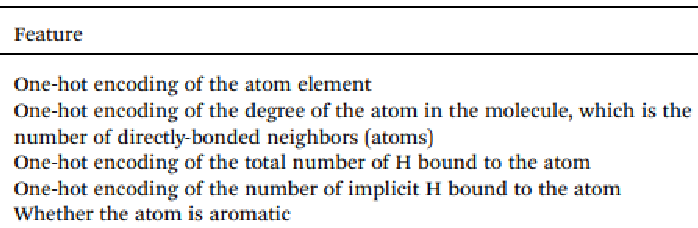
\includegraphics[width=1.0\linewidth]{images/Jiang_Atom_Node_Features.pdf}
  \caption{Part of a table taken from \citet{Jiang2020} showcasing the atom node features used.}
  \label{tbl:Jiang_Atom_Node_Features}
\end{table}

\begin{table}[!h]
  \centering
  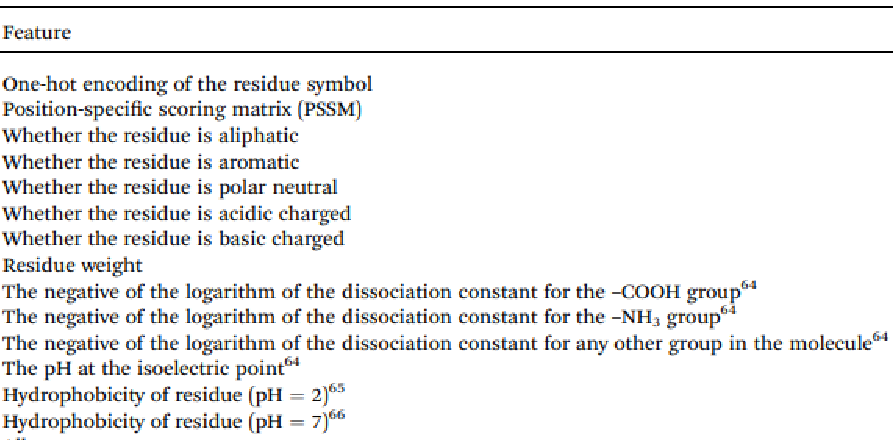
\includegraphics[width=1.0\linewidth]{images/Jiang_Residue_Node_Features.pdf}
   \caption{Part of a table taken from \citet{Jiang2020} showcasing the residue node features used.}
  \label{tbl:Jiang_Residue_Node_Features}
\end{table}

\pagebreak

\subsection{Valuable Strategies \& Concepts}

All studies highlighted that the complicated structure of proteins and molecules make the creation of accurate representations, the features that will be passed into the models, one of the hardest parts of the whole process. This is an active area of research in it of itself in computer-aided medicine. \citep{Jiang2020}

Both \citet{Jiang2020} and \citet{Gligorijević} agree that the most efficient way to process a protein 3D structure is with a GCN as it generalises convolutional operations on efficient graph-like molecular representations. GCNs have also shown vast success in problems such as the prediction of biochemical activity of drugs and prediction of interfaces between pairs of proteins \citep{Gligorijević}.